
\documentclass[10pt,onecolumn]{RequimentsGathering}

% All KJN's macros and goodies (some shameless borrowing from SPL)
\usepackage{KJN}

%\usepackage[hyphens]{url}

% PDF Info
%
\ifpdf
\pdfinfo{
	/Title (SOFTWARE ENGINEERING PROJECT: STUDENTS MARKS/RECORDS MANAGEMENT SOFTWARE)
	/Author (Khosa Masana (559990), Sanele Gcaba(459380), Tshegofatso Misapitso (600313), Londiwe Ngema (448871) )
	/ModDate (D:200510121530)
	/Subject (ELEN417/455 Paper Format, 2005)
	/Keywords (ELEN417, ELEN455, paper, instructions, style guidelines, laboratory project)
}
\fi

%%%%%%%%%%%%%%%%%%%%%%%%%%%%%%%%%%%%%%%%%%%%%%%%%%%%%%%%%%%%%%%%%%%%%%%%%%%%%%%
\begin{document}
	
	\begin{titlepage}
		
		\newcommand{\HRule}{\rule{\linewidth}{0.5mm}} % Defines a new command for the horizontal lines, change thickness here
		
		\center % Center everything on the page
		{\small School$\;$of$\;$Electrical$\;$and$\;$Information$\;$Engineering,$\;$University of$\;$the$\;$Witwatersrand,$\;$Private$\;$Bag$\;$3,$\;$2050,$\;$Johannesburg,$\;$South$\;$Africa}\\[1.5cm] % Name of your university/college
		
		\textsc{ELEN 4009 - Software Engineering}\\[0.5cm] % Major heading such as course name
		
		\HRule \\[0.4cm]
		{ \large \bfseries Student Marks/Records Management Software - Requirements Gathering}\\[0.4cm] % Title of your document
		\HRule \\[1.5cm]
		
		\large
		
		\textbf{Project Team :}
		Khosa$\;$Masana$\;$(559990),
		Sanele$\;$Gcaba$\;$(459380),
		Tshegofatso$\;$Misapitso$\;$(600313) and
		Londiwe$\;$Ngema$\;$(448871)
		
		
		{\large \today}\\[3cm] % Date, change the \today to a set date if you want to be precise
		
		%\includegraphics{Logo}\\[1cm] % Include a department/university logo - this will require the graphicx package
		
		\vfill % Fill the rest of the page with whitespace
		
	\end{titlepage}
	
	\pagestyle{plain}.
	\pagenumbering{roman} 
	\tableofcontents 
	
	\newpage
	
	\section*{Document Status Sheet}
	
	\begin{center}
		\begin{tabular}{ | p{5cm} | p{7cm} |}
			\hline
			\textbf{Document Title}& Software Requirements\\ \hline
			\textbf{Authors} & M.$\;$Khosa, S.$\;$Gcaba, T.$\;$Misapitso, L.$\;$Ngema \\ \hline
			\textbf{Version} & 0.01 \\ \hline
			\textbf{Document Status} & Draft  \\ \hline
			
		\end{tabular}
	\end{center}
	
	
	\begin{center}
		\begin{tabular}{ | p{2cm} | p{3cm} | p{5cm} | p{5cm} |}
			\hline
			\textbf{Version}& \textbf{Date}& \textbf{Author(s)} & \textbf{Summary} \\ \hline
			0.0.1 & 25-02-2016 & M.$\;$Khosa, S.$\;$Gcaba, T.$\;$Misapitso, L.$\;$Ngema& Document Creation. \\ \hline
			
		\end{tabular}
	\end{center}
	
	\newpage
	
	
	%%%%%%%%%%%%%%%%%%%%%%%%%%%%%%%%%%%%%%%%%%%%%%%%%%%%%%%%%%%%%%%%%%%%%%%%%%%%%%%
	%
	\pagestyle{plain}.
	\pagenumbering{arabic} 
	\section{Introduction}

\subsection{Methodology}

The System Development Life Cycle (SDLC) methodology to be used for the project follows the Agile Model, this models breaks down the product into a cycle, it quickly delivers a working product and is a more realistic methodology. Ongoing releases are produced with small incremental changes and it depends heavily on customer interaction \cite{ref7}. Specifically the Scrum Agile Model will be adopted for the project, Scrum comprises of short sprints and it enables the software team to be able to prioritize on what matters most. It is basically about delivering more often and getting feedback what is regularly responded to \cite{ref8}.           

\subsection{Purpose}

The purpose of this document is to present a detailed description of the requirements for the student marks/record system (SMMS). It will state the purpose and features of the system, the interfaces of the system, what the system will do, the limitations under which it must operate, define inputs and the expected reaction of the system (that is the outputs of the system). 

Student Marks/Records Management Software provides on-line services that enable students to view their marks as they complete  assignments, tests and laboratory work, the software system allows staff such as course coordinators the right to add/edit marks obtained by the student under different forms of assessment. It is a convenient way for students to have access to their marks in a safe and confidential way as opposed to accessing them on notice boards where everyone else can publicly see them. The system ensures that each student can track his/her tentative progress throughout the year,it also helps in establishing errors in the record as early as possibly. 

\subsection{Project Scope}
\begin{itemize}

\item There are three basic users of the system - Students, Course coordinators and School administrator.
\item The primary function of the application is to allow students and staff  to log-in using their details (Student/Staff number and password) and be able to access and view student records, the records include student marks for all forms of assessments for all courses registered for. 
\item The system database stores user profiles and student marks records. Marks records are retained for a period of 10 yrs.
\item The software program should have domains assigned, i.e. each user can be able to access relevant  information and they are allowed to view/edit/add based on what their recognised  domain.
\item  The system would be accessed online via a Browser and/or a Smart-phone App.

\end{itemize}

Below is a list of privileges per user as specified on the project brief \cite{ref9}.

\textbf{The Course Coordinator should be able to:-}
\begin{itemize}
\item Register himself/herself.
\item Add various assessment method for the course and weighting for each assessment.
\item Enter student marks on a user-friendly interface.
\item Display or print out the table of students and their marks.
\item Generate a summary statistics of the performance of the students - maximum, minimum, average, standard deviation or variants of each assessment.  
\item View projected pass rate based on the assessment marks accumulated students in class.
\end{itemize}

\textbf{The School Administrator should be able to:-}
\begin{itemize}
\item Register himself/herself.
\item Display or print out table of students and their marks.
\item Generate a summary statistics of the performance f the students. 
\item Generate a comparative chart of the assessment marks of selected courses being taken by students of a particular group. 
\item Histogram of assessment marks of all courses taken a specific student.   
\item Any recorded offences (e.g. plagiarism) for a student.
\item The performances in the same course across different years may be compared.
\end{itemize}

\textbf{The Student should be able to:-}
\begin{itemize}
\item Register himself/herself.
\item Display assessment marks for a course and statistics for that assessment.
\item Display assessment marks for all the courses  
\item Based on current assessment marks, give what performance goals are needed to pass the course.
\end{itemize}

\subsection{List of Definitions and abbreviations}

\subsubsection{Definitions}
\begin{center}
    \begin{tabular}{ | p{3cm} | p{9cm} |}
\hline
\textbf{Term}& \textbf{Definition}\\ \hline
 Database & A collection of records stored within the system \\ \hline
 Table & A collection of related data consisting of columns and rows \\ \hline   
     \end{tabular}
\end{center}

\subsubsection{Abbreviations}

\textbf{SMMS} - Student Marks/record management system

\textbf{HTTP} - Hypertext Transfer Protocol

\textbf{HTML} - HyperText Markup Language

\textbf{RDBMS} - Relational Database Management System

\textbf{SQL} - Structured Query Language

%%%%%%%%%%%%%%%%%%%%%%%%%%%%%%%%%%%%%%%%%%%%%%%%%%%%%%%%%%%%%%%%%%%%%%%%%%%%%%%
%
\subsection{Tools used}
\textbf{Web server} - Apache2

The Apache web server is the worlds most used web server software program, it uses HTTP to serve files that form web pages to users in response to their requests. It is an open source program \cite{ref5, ref6}. 

\textbf{Development tools (Front-End)} - HTML, CSS and Javascript

\textbf{Development tools (Back-End)} - PHP 

PHP is a server scripting language, it is widely used, free, and efficient tool.

\textbf{Database Platform} - MySQL and PHPmyadmin 

MySQL is an open-source RDBMS, it stores data in tables and PHPmyadmin is a graphical tool intended to handle administration of MySQL over the web.   

\subsection{Programs to install}

To run the above mentioned programs these are the softwares to install: PHP, MySql and Apache.
\section{Expanded Description of the project}

The software system will follow a Two-Tier Architecture due to its ease of use and maintainability as compared to a Three-Tier Architecture. However, the performance of a Two-Tier Architecture slows down with an increase in users \cite{ref3}, hence a Three-Tier Architecture will be implemented with an increase of the number of users. Figure 1 below shows the Two-Tier Architecture.   
\begin{center}
\begin{figure}[h]
\centering
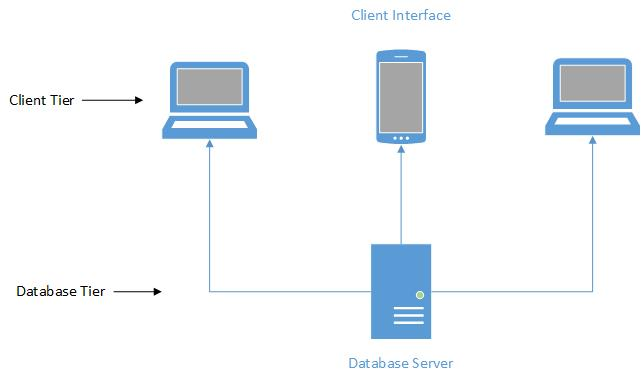
\includegraphics[width=10cm]{Two-Tier}
\caption{Two-Tier Software Architecture}
\end{figure}
\end{center}


A Two-Tier Architecture is a software architecture where the interface runs on client and the data layer is stored on a server\cite{ref4}.

\section{Overall Description}	

\subsection{Constraints }
\begin{itemize}
\item The User Interface language is English only.
\item Students cannot view test marks, only the final marks.
\end{itemize}


\subsection{ER Diagrams }
The ER Diagrams show how data is organized within the database.

\begin{center}
\begin{figure}[h]
\centering
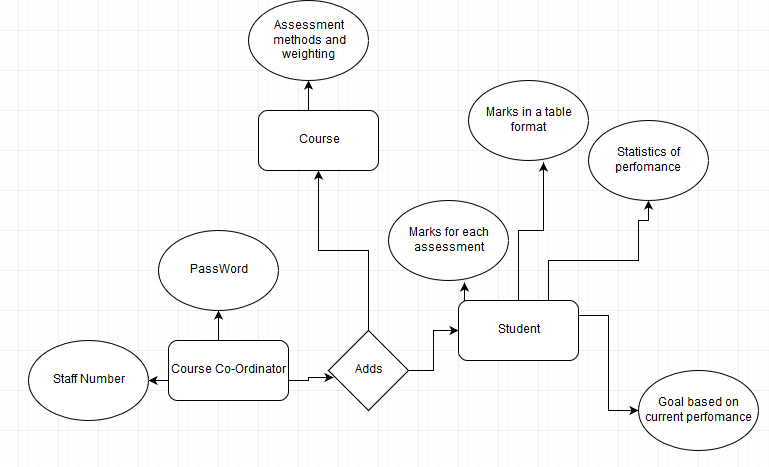
\includegraphics[width=10cm]{ER1}
\caption{ER Diagram for Course co-ordinator and student}
\end{figure}
\end{center}

\begin{center}
\begin{figure}[h]
\centering
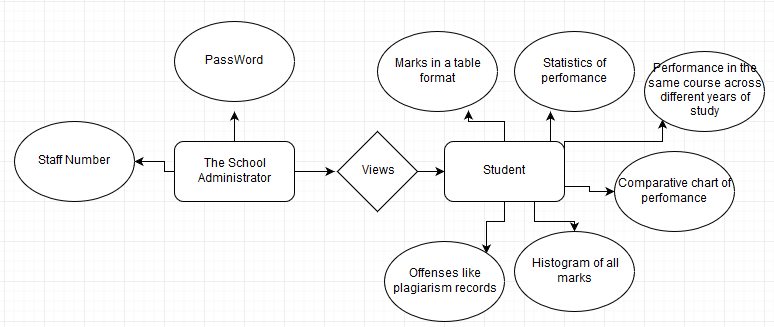
\includegraphics[width=10cm]{ER2}
\caption{ER Diagram for the administrator and student}
\end{figure}
\end{center}

\newpage

\begin{center}
\begin{figure}[h]
\centering
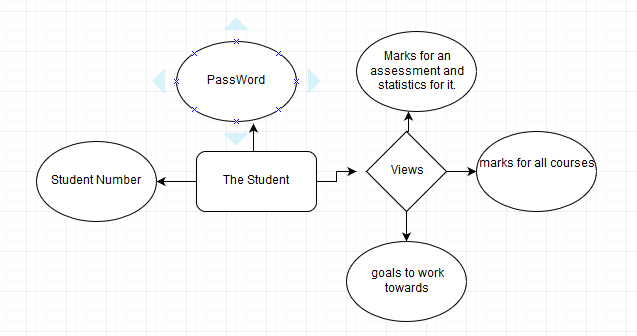
\includegraphics[width=10cm]{ER3}
\caption{ER Diagram for student}
\end{figure}
\end{center}

\newpage
\subsection{Hardware Specifications }
\textbf{Minimum Requirements}
\begin{center}
	\textbf{Client side}\\
	\begin{tabular}{ | p{5cm} | p{4cm} | p{3cm} | p{3cm} |}
		\hline
		\textbf{Windows} & \textbf{Processor} & \textbf{RAM} & \textbf{Disk Space}\\ \hline
		Internet Explorer	&	Intel Pentium III	
		or AMD - 800 MHz	&	128 MB	&	100 MB		\\ \hline
		Google Chrome		&	Intel Pentium IV - 
		SSE2 capable		&	128 MB	&	100 MB		\\ \hline
	\end{tabular}
	
	
	\begin{tabular}{ | p{5cm} | p{4cm} | p{3cm} | p{3cm} |}
		\hline
		\textbf{Mac} & \textbf{Processor} & \textbf{RAM} & \textbf{Disk Space}\\			\hline
		Google Chrome		&	64 bit Intel  
		processor	       &   128 MB  &	100 MB	\\ \hline
	\end{tabular}
	
	
	\begin{tabular}{ | p{5cm} | p{4cm} | p{3cm} | p{3cm} |}
		\hline			\textbf{Linux} & \textbf{Processor} & \textbf{RAM} & \textbf{Disk Space}\\
		\hline
		Google Chrome		&	Intel Pentium III  
		processor	       &   128 MB  &	100 MB	\\ \hline
	\end{tabular}
	
	\textbf{Server side}\\
	\begin{tabular}{ | p{5cm} | p{4cm} | p{3cm} | p{3cm} |}
		\hline	
		\textbf{Linux} & \textbf{Processor} & \textbf{RAM} & \textbf{Disk Space}\\
		\hline
		Apache 2		&	2 GHz processor or faster  
		processor	       &   1 GB (32 bit) or 2 GB (64 bit)  &		\\ \hline
	\end{tabular}
\end{center}

\textbf{Recommended Requirements}
\begin{center}
	\textbf{Client side}\\
	\begin{tabular}{ | p{5cm} | p{4cm} | p{3cm} | p{3cm} |}
		\hline
		\textbf{Windows} & \textbf{Processor} & \textbf{RAM} & \textbf{Disk Space}\\ \hline
		Internet Explorer	&	1 GHz or faster	&	1 GB (32 bit) or 2 GB (64 bit)	&	256 MB		\\ \hline
	\end{tabular}
	
	
	\begin{tabular}{ | p{5cm} | p{4cm} | p{3cm} | p{3cm} |}
		\hline
		\textbf{Mac} & \textbf{Processor} & \textbf{RAM} & \textbf{Disk Space}\\				\hline
		Google Chrome	&	64 bit Intel processor	 &  1 GB  &	256 MB	\\ \hline
	\end{tabular}
	
	
	\begin{tabular}{ | p{5cm} | p{4cm} | p{3cm} | p{3cm} |}
		\hline
		\textbf{Linux} & \textbf{Processor} & \textbf{RAM} & \textbf{Disk Space}\\
		\hline
		Google Chrome		1 GHz or faster	&	1 GB (32 bit) or 2 GB (64 bit)	&	256 MB	\\ \hline
	\end{tabular}
	
	
	\textbf{Server side}
	Server specifications will depend on the development of the project.
\end{center}

	
	\section{Specific Requirements}
	
	\subsection{UML Activity Diagram}
	
	Figure 2 Shows the UML activity diagram of the how the software should work. As shown in the UML activity diagram, the user will first be ask to enter a user-name and a password. This is done to keep track of the type of user who will be interacting with the software i.e student, staff and admin. Each type of user will be given different rights to interact with the server as shown in the UML diagram. Students are only allowed to view the results, staff is allowed to change marks or add results and the administrator will be responsible of adding or removing users.   
	
	\begin{center}
		\begin{figure}[h]
			\centering
			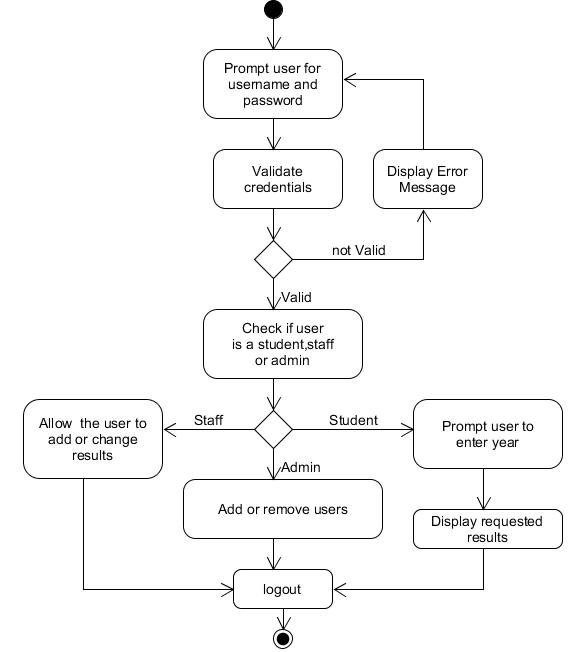
\includegraphics[trim={0cm 0 0 0},clip]{UML-Activity}
			\caption{UML Activity Diagram}
		\end{figure}
	\end{center}
	
	\subsection{Use Case Reports}
	Since we have only three users of the software, namely student, staff and administrator, three use case reports have been made for each user. 
	
	
	\subsection{Use Case Reports (Masana Khosa)}
	Since we have only three users of the software, namely student, staff and administrator, three use case reports have been made for each user. 
	
	
	\clearpage
	\subsubsection{Student Use-Case Report}$\;\;\;\;\;\;\;\;\;\;\;\;\;\;\;\;\;\;\;\;\;\;\;$
	
	A use case report for a student is shown in Figure 3.
	\begin{center}
		\begin{figure}[h]
			\centering
			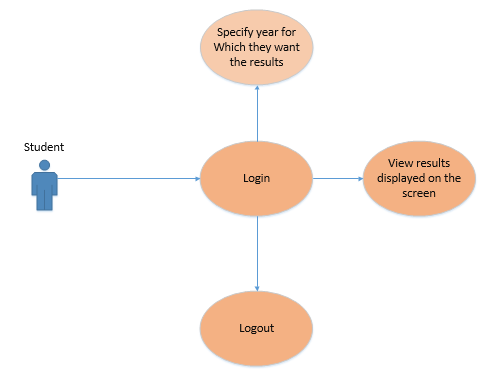
\includegraphics[trim={0cm 0cm 0cm 0cm },clip,scale = 1.1]{StudentUsecase}
			\caption{Use Case Diagram For Student}
		\end{figure}
	\end{center}
	
	
	
	\begin{center}
		\begin{tabular}{ | p{3cm} | p{10cm}| }
			\hline
			\textbf{Use case}& \textbf{Description} \\ \hline
			Register & The student need to sign in in order to view the results \\ \hline
			Display assessment marks & A student must be to display assessment marks for all courses  \\ \hline
			Statistics for an assessment & A student must be able to display assessment marks for a course and the statistics for that assessment \\ \hline
			View performance goals & A student must be able to view what perfomance goals are needed to pass pass the course based on current assessment \\ \hline
			Logout          & The student must be able to logout  \\ \hline
			
		\end{tabular}
	\end{center}
	\clearpage
	\subsubsection{Course Coordinator Use-Case Report}$\;\;\;\;\;\;\;\;\;\;\;\;\;\;\;\;\;\;\;\;\;\;\;$
	
	A use case report for Course Coordinator is shown in Figure 4.
	\begin{center}
		\begin{figure}[h]
			\centering
			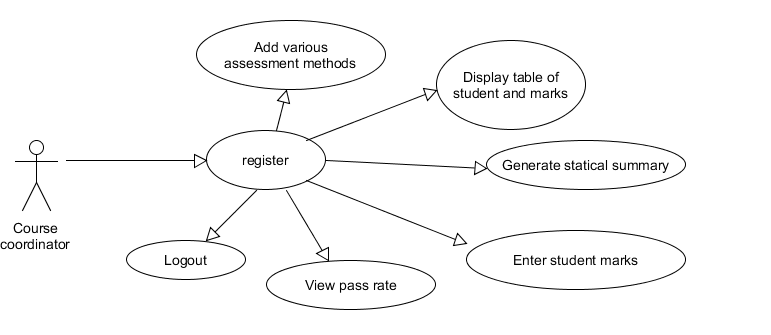
\includegraphics[trim={0cm 0cm 0cm 0cm },clip,scale = 0.85]{CourseCoordinatorUsecase}
			\caption{Use Case Diagram For Staff}
		\end{figure}
	\end{center}
	
	
	
	\begin{center}
		\begin{tabular}{ | p{3cm} | p{10cm}| }
			\hline
			\textbf{Use case}& \textbf{Description} \\ \hline
			Register & Staff need to sign in order to modify results \\ \hline
			Add various assessment methods & Add various assessment method for the course and the weighting for each assessment  \\ \hline
			
			Display table of student and marks & Display or print out the table
of studets and their marks\\ \hline
            Generate statical summary & Generate A summary statistics of the perfomance of each student  \\ \hline
            Enter student marks & Enters the student's marks for each assessment in a user-friendly interface \\ \hline
            View pass rate & View projected pass rate based on the assessment marks accumulated by the students in the class thus far \\ \hline
			Logout          & Coordinator member must be able to logout  \\ \hline
			
		\end{tabular}
	\end{center}
	
	
	
	
	\clearpage
	\subsubsection{Administrator Use-Case Report}$\;\;\;\;\;\;\;\;\;\;\;\;\;\;\;\;\;\;\;\;\;\;\;$
	
	A use case report for an Administrator is shown in Figure 5.
	\begin{center}
		\begin{figure}[h]
			\centering
			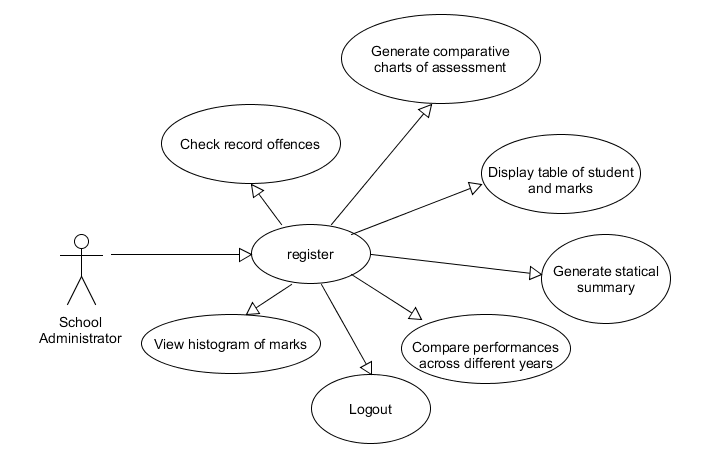
\includegraphics[trim={0cm 0cm 0cm 0cm },clip,scale = 0.85]{AdminUsecase}
			\caption{Use Case Diagram For Administrator}
		\end{figure}
	\end{center}
	
	
	
	\begin{center}
		\begin{tabular}{ | p{3cm} | p{10cm}| }
			\hline
			\textbf{Use case}& \textbf{Description} \\ \hline
			Register & Administrator need to sign in \\ \hline
			Check record offences & The administrator must be able to check any record offences like plagiarism for a student   \\ \hline
			Generate comparative charts of assessment & Generate a comparative chart of the assessment marks of selected courses 
being taken by students of a particular group \\ \hline
Display table of student and marks & Display or print out the table
of studets and their marks\\ \hline
Generate statical summary & Generate A summary statistics of the perfomance of each student  \\ \hline
Compare performances across different years & compare performances in the same course across different years \\ \hline 
View histogram of marks & View a histogram of assessment marks
of all courses taken by a specific specific student  \\ \hline 

			Logout          & Administrator must be able to logout  \\ \hline
			
		\end{tabular}
	\end{center}
	
	
	\section{Sequence Diagram}
	
	The sequence diagram in Figure 11 shows Sequence diagram of a student.  
	
	
	\begin{center}
		\begin{figure}[h]
			\centering
			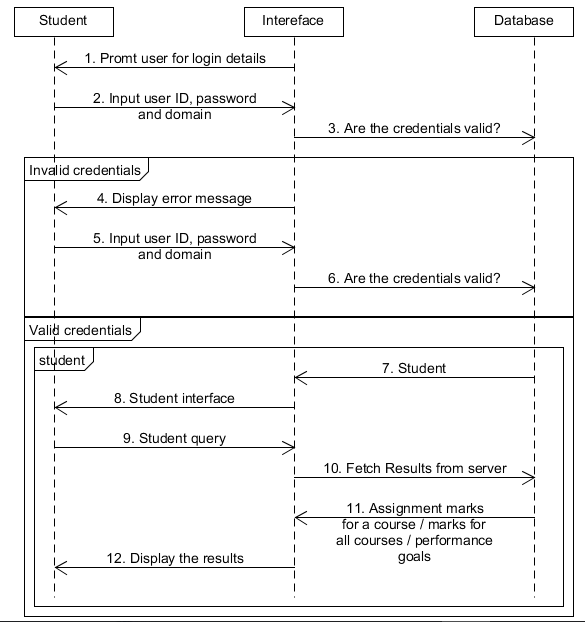
\includegraphics[trim={0cm 0cm 0cm 0cm },clip,scale = 1.1]{StudentSequence}
			\caption{Student Sequence Diagram}
		\end{figure}
	\end{center}
	\newpage
	
	
	The sequence diagram in Figure 12 shows Sequence diagram of an administrator.  
	
	
	\begin{center}
		\begin{figure}[h]
			\centering
			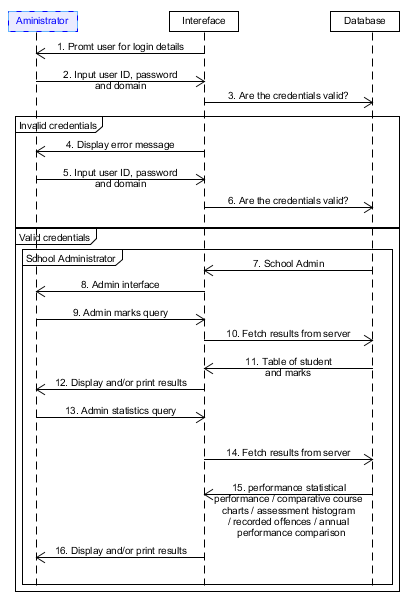
\includegraphics[trim={0cm 0cm 0cm 0cm },clip,scale = 1.1]{AdministratorSequence}
			\caption{ Administrator Sequence Diagram}
		\end{figure}
	\end{center}
	\newpage
	
		The sequence diagram in Figure 13 shows Sequence diagram of an course coordinator.  
	
	
	\begin{center}
		\begin{figure}[h]
			\centering
			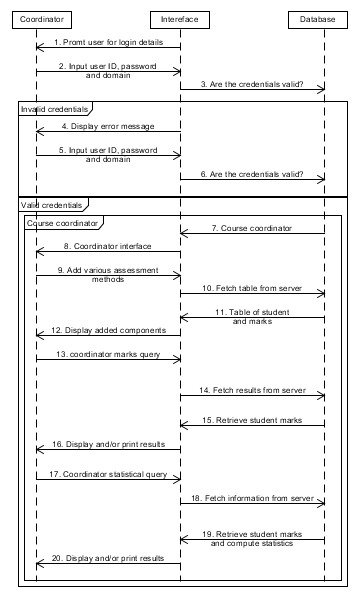
\includegraphics[trim={0cm 0cm 0cm 0cm },clip,scale = 1.1]{CoordinatorSequence}
			\caption{Course Coordinator Sequence Diagram}
		\end{figure}
	\end{center}
	\newpage
	
\section{Responsibilities And The current prototype}

\subsection{Front-End}

Masana Khosa and Londiwe Ngema are responsible for the front end, they designed the website page and the interfaces for the individual users. They also created domains to ensure that the user only has access to what they need. The current prototype allows users to log in and they are redirected to the different pages based on the scope above. Since there are different types of users with different privileges, they are distinguished using a domain. A student cannot log on the system as a stuff member and vice versa. When a user logs out they are directed to the home page.

\subsection{Back-End}

Sanele Gcaba and Tshegofatso Misapitso are responsible for the back end that is the database. The next step is to do the querying logic to link the back and front ends. The program is now able to log the registered users in and out based on the information from the database. Different interfaces can now be called upon for different users, i.e different interfaces for the school administrator, course co-ordinator and the students.


The developed Back-End constitute of a LAMP web server, this is hosted within a PC and accessible using a local host of a machine. The server that hosts the database was created using PHPmyadmin. The Back-end now has a database for users, it has a Username, Password and Domain. The back-end team has been able ensure a link between the front end interface and the login database. 


The back-end:
The proposed design of the back-end is to include a Linux Apache MySQL PHP(LAMP) installation.

The Linux operating system is chosen for the server to run on because of its Stability, Security and Cost of operation \cite{ref1}.   
As a result Linux Mint operating system was chosen.
The Linux is Just the base of the project that will allow the server to run off. The server proposed is an Apache server. This server is chosen because it is easy to install and operate. Apache will provide a secure, efficient and extensible server that provides HTTP services.
The project requires that data is stored and later on read from. There is multiple datasets that need to be considered: for example multiple students that may be doing multiple courses and as a result a need for storing this data. MySQL was chosen because it is an open source database and large companies use it to save money and time powering their high volume websites \cite{ref2}.

PHP is  selected as a server the scripting language. This is chosen because of the simplicity of the language and in addition JavaScript can be used to do client side validation to avoid overloading the server with server side validation. Validation would be necessary for authentication. 

PHPMyadmin may be used in order to get a visual look of the database instead of having to type out queries in order to check that the data one expects to be in the database is actually in the database. 
Interacting: the client tries logging in:

\begin{itemize}
\item Client enters credentials, these credentials get validated ‘onsubmit’.
\item If the credentials are correct: a PHP script is used to determine if the user is a  student or staff member.
\item If the user is a student then the student will only have certain privileges such as reading from the database only.
\item If the user is an administrator or a staff member then they may be allowed to have different privileges to edit the database: such as alter student results and add new student onto the database.
\end{itemize}


Figure below shows the user database design.

\newpage

\begin{center}
\begin{figure}[h]
\centering
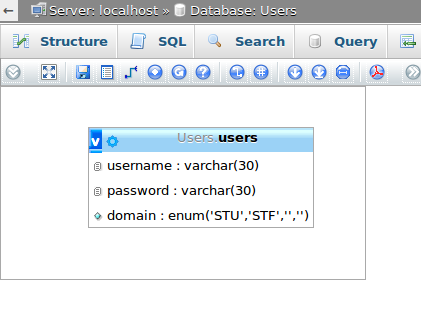
\includegraphics[width=10cm]{Users}
\caption{User Database}
\end{figure}
\end{center}
     
Additionally a student record Database was created and a figure below shows a structure for the database

\begin{center}
\begin{figure}[h]
\centering
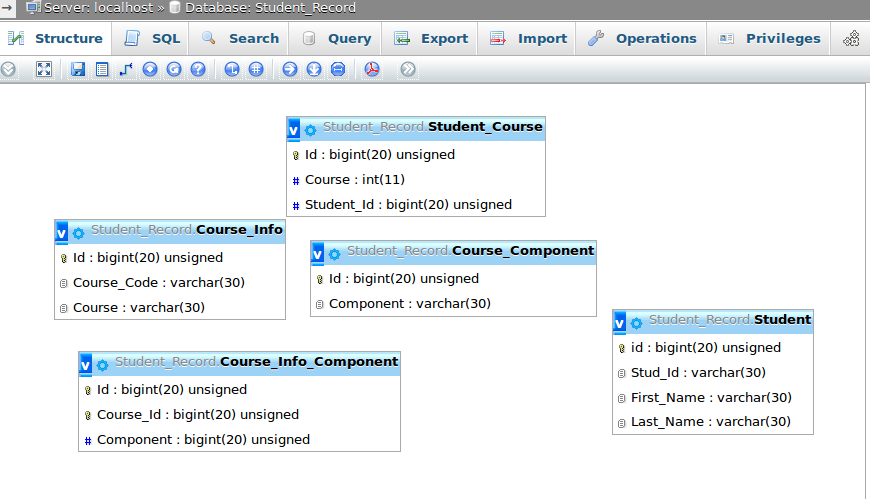
\includegraphics[width=10cm]{StudentRecord}
\caption{Student Record Database}
\end{figure}
\end{center}

\newpage
	
	\vfill
	
	%\nocite{*}
	\bibliographystyle{witseie}
	\bibliography{sample}
	
	%{\tiny \vfill \hfill \today \hspace{5mm} witseie-paper-2003.\TeX}
	
\end{document}

" vim: ts=4
" vim: tw=78
" vim: autoindent
" vim: shiftwidth=4
